\chapter[Leçon 41: Phonetik, Diphthongen, Vokallängt \& Reesen]{Leçon 41: Alldagskonversatioun, Diphthongen, kuerz a laang Vokalen, Reesen \& Beruff}

Dës Lektioun verbënnt alldeeglech Gespréichsthemen (\textbf{Beruff, Gesondheet, Reparaturen a Reesen}) mat engem déiwe Bléck op d'\textbf{Lëtzebuerger Phonetik an Orthografie}. Mir léiere fir d'éischt Vokabulär ronderëm Beruff a Fuerschung (\textit{Hiewan}, \textit{Fuerscherin}, \textit{en Doktorat maachen}) souwéi nëtzlech Ausdréck fir \textit{Repair Café}, Gesondheet an d'Konjunktioun \textbf{awer} vs. \textbf{oder}. Duerno schaffe mir mat engem klassesche Liesziedel (\textit{Lieszeechen}), fir all déi wichteg \textbf{Diphthongen} (\textit{oi, ou, ei, éi, ai, äi, au}) an d'\textbf{Reegelen tëscht kuerzen a laange Vokalen} (\textit{bal} vs. \textit{Ball}, \textit{Kap} vs. \textit{Kapp}, \textit{Aarbecht}) sécher ze beherrschen. Zum Schluss übe mir wichteg Verben (\textit{bleiwen, leien, flécken, reesen, fueren, maachen}) an typesch \textbf{Sproochentest-Froen iwwer d'Reesen an d'Vakanz}.

\textit{Cette leçon associe des thèmes de conversation quotidienne (\textbf{professions, santé, réparations et voyages}) à une étude approfondie de la \textbf{phonétique et de l'orthographe luxembourgeoises}. Nous abordons d'abord le vocabulaire des professions et de la recherche (\textit{Hiewan} sage-femme, \textit{Fuerscherin} chercheuse, \textit{en Doktorat maachen}), ainsi que des expressions utiles autour du \textit{Repair Café}, de la santé et la différence entre \textbf{awer} (mais) et \textbf{oder} (ou). Ensuite, nous travaillons à l'aide d'un marque-page phonétique pour maîtriser toutes les \textbf{diphtongues} (\textit{oi, ou, ei, éi, ai, äi, au}) et les \textbf{règles de longueur des voyelles} (\textit{bal} vs \textit{Ball}, \textit{Kap} vs \textit{Kapp}, \textit{Aarbecht}). Enfin, nous pratiquons la conjugaison de verbes clés (\textit{bleiwen, leien, flécken, reesen, fueren, maachen}) et des questions types du \textbf{Sproochentest sur les voyages et les vacances}.}

\textit{This lesson combines everyday conversation topics (\textbf{professions, health, repairs, and travel}) with a thorough look at \textbf{Luxembourgish phonetics and spelling}. First, we cover vocabulary related to professions and research (\textit{Hiewan} midwife, \textit{Fuerscherin} researcher, \textit{en Doktorat maachen}), along with useful expressions for a \textit{Repair Café}, health, and the conjunctions \textbf{awer} (but) vs. \textbf{oder} (or). Next, we use a classic phonetic bookmark to master all major \textbf{diphthongs} (\textit{oi, ou, ei, éi, ai, äi, au}) and the \textbf{rules for short vs. long vowels} (\textit{bal} vs. \textit{Ball}, \textit{Kap} vs. \textit{Kapp}, \textit{Aarbecht}). Finally, we practice key verbs (\textit{bleiwen, leien, flécken, reesen, fueren, maachen}) and typical \textbf{Sproochentest questions about travel and holidays}.}

\vspace{1.5em}

% ==============================================================================
% SECTION I: ALLDAGSGESPRÉICHER: BERUFF, GESONDHEET A REPARATUREN
% ==============================================================================
\section[Alldagsgespréicher : Beruff, Gesondheet a Reparaturen]{Alldagsgespréicher : Beruff, Gesondheet a Reparaturen \\/ Conversations du quotidien : métier, santé et réparations \\/ Everyday Conversations: Profession, Health and Repairs}

\subsection{Beruff a Fuerschung : vun der \textit{Hiewan} zur \textit{Fuerscherin}}

\begin{itemize}
    \item \textbf{D'Hiewan (f., Pl. d'Hiewanen / d'Hiewannen) -- la sage-femme / the midwife} \\
    \textbf{D'Fuerscherin (f., Pl. d'Fuerscherinnen) -- la chercheuse / the researcher} \\
    \textit{FR : En luxembourgeois, « sage-femme » se dit \textbf{d'Hiewan} et « chercheuse » se dit \textbf{d'Fuerscherin} (du verbe \textbf{fuerschen}, faire de la recherche).} \\
    \textit{EN : In Luxembourgish, "midwife" is \textbf{d'Hiewan} and "researcher" is \textbf{d'Fuerscherin} (from the verb \textbf{fuerschen}, to do research).}
    \begin{itemize}
        \item \textit{An Italien hunn ech als \textbf{Hiewan} am \textbf{Spidol} geschafft.} \\
        $\rightarrow$ \textit{FR :} En Italie, j'ai travaillé comme sage-femme à l'hôpital. \\
        $\rightarrow$ \textit{EN :} In Italy, I worked as a midwife at the hospital.
        \item \textit{Elo wëll ech als \textbf{Fuerscherin} op der \textbf{Universitéit Lëtzebuerg} schaffen an iwwer d'Hiewane-Beruffsbild \textbf{fuerschen}.} \\
        $\rightarrow$ \textit{FR :} Maintenant, je veux travailler comme chercheuse à l'Université du Luxembourg et faire des recherches sur la profession de sage-femme. \\
        $\rightarrow$ \textit{EN :} Now I want to work as a researcher at the University of Luxembourg and do research on the midwifery profession.
    \end{itemize}

    \vspace{0.3em}

    \item \textbf{Nëtzleche Vocabulaire :}
    \begin{itemize}
        \item \textbf{d'Spidol} (n., Pl. \textit{d'Spideeler}) -- l'hôpital / the hospital
        \item \textbf{den Doktorat} (m.) / \textbf{en Doktorat maachen} -- le doctorat / to do a PhD
        \item \textbf{op der Universitéit schaffen} -- travailler à l'université / to work at the university
        \item \textbf{mat der Universitéit schwätzen} -- parler avec l'université / to speak with the university
    \end{itemize}
\end{itemize}

\subsection{Gesondheet a Reparaturen : \textit{krank sinn}, \textit{futti} a \textit{flécken}}

\begin{itemize}
    \item \textbf{Iwwer d'Gesondheet schwätzen (Parler de la santé / Talking about health) :}
    \begin{itemize}
        \item \textit{Wéi geet et dir ? -- Net gutt. Ech war \textbf{krank}, eng ganz Woch (oder : dräi Wochen) !} \\
        $\rightarrow$ \textit{FR :} Comment vas-tu ? -- Pas bien. J'ai été malade toute une semaine (ou : trois semaines) ! \\
        $\rightarrow$ \textit{EN :} How are you? -- Not good. I was sick for a whole week (or: three weeks)!
        \item \textit{Wars du net krank ? -- Nee, mir geet et gutt.} \\
        $\rightarrow$ \textit{FR :} Tu n'as pas été malade ? -- Non, je vais bien. \\
        $\rightarrow$ \textit{EN :} Weren't you sick? -- No, I am doing well.
    \end{itemize}

    \vspace{0.3em}

    \item \textbf{Reparaturen a Repair Café (Réparations et Repair Café / Repairs and Repair Café) :}
    \begin{itemize}
        \item \textit{Mäin Autoradio ass \textbf{futti} (oder : \textbf{blockéiert / gespaart}). Ech hu mäi Code vergiess !} \\
        $\rightarrow$ \textit{FR :} Mon autoradio est cassé (ou : bloqué). J'ai oublié mon code ! \\
        $\rightarrow$ \textit{EN :} My car radio is broken (or: blocked / locked). I forgot my code!
        \item \textit{Wann eppes \textbf{futti} ass (zum Beispill eng Auer oder e Radio), kann een an e \textbf{Repair Café} goen : d'Benevollen \textbf{flécken} et.} \\
        $\rightarrow$ \textit{FR :} Quand quelque chose est cassé (par exemple une montre ou une radio), on peut aller dans un Repair Café : les bénévoles le réparent. \\
        $\rightarrow$ \textit{EN :} When something is broken (for example a watch or a radio), you can go to a Repair Café: the volunteers repair it.
    \end{itemize}

    \vspace{0.3em}

    \item \textbf{Grammatesch Notiz : \textit{awer} (mais / but) vs. \textit{oder} (ou / or) :} \\
    Verwiesselt net déi zwou Konjunktiounen : \textbf{awer} bedeit « mais / but » (net dat däitscht \textit{*aber}), an \textbf{oder} bedeit « ou / or ». \\
    \textit{FR : Ne confondez pas \textbf{awer} (« mais », et non l'allemand *aber) avec \textbf{oder} (« ou »).} \\
    \textit{EN : Do not confuse \textbf{awer} ("but", not German *aber) with \textbf{oder} ("or").}
    \begin{itemize}
        \item \textit{Ech schaffe gär hei, \textbf{awer} am Dezember schwätzen ech mat der Universitéit.} \\
        $\rightarrow$ \textit{FR :} J'aime travailler ici, mais en décembre je parle avec l'université. \\
        $\rightarrow$ \textit{EN :} I like working here, but in December I am speaking with the university.
        \item \textit{Schaffs du an engem Spidol \textbf{oder} op der Universitéit ?} \\
        $\rightarrow$ \textit{FR :} Travailles-tu dans un hôpital ou à l'université ? \\
        $\rightarrow$ \textit{EN :} Do you work in a hospital or at the university?
    \end{itemize}
\end{itemize}

\vspace{1.5em}

% ==============================================================================
% SECTION II: D'DIPHTHONGEN OP LËTZEBUERGESCH
% ==============================================================================
\section[D'Diphthongen op Lëtzebuergesch]{D'Diphthongen op Lëtzebuergesch (Lieszeechen) \\/ Les diphtongues en luxembourgeois \\/ Diphthongs in Luxembourgish}

Fir d'Aussprooch vun de Lëtzebuerger Diphthongen ze üben, sinn déi siwe Sätz vum Liesziedel ideal. All Saz weist een typeschen Diphthong : \\
\textit{FR : Pour pratiquer la prononciation des diphtongues luxembourgeoises, les sept phrases du marque-page sont idéales. Chaque phrase illustre une diphtongue caractéristique :} \\
\textit{EN : To practice the pronunciation of Luxembourgish diphthongs, the seven sentences from the phonetic bookmark are ideal. Each sentence illustrates a characteristic diphthong:}

\begin{table}[htbp]
    \centering
    \small
    \begin{tabular}{llp{5.5cm}p{5.2cm}}
        \toprule
        \textbf{Diphthong} & \textbf{IPA} & \textbf{Beispillsaz} & \textbf{Iwwersetzung (FR / EN)} \\
        \midrule
        \textbf{oi} & {[oɪ]} & \textbf{Moien !} & Bonjour ! / Hello! \\
        \textbf{ou} & {[əʊ]} & \textbf{Wou ass déi rout Kou ?} & Où est la vache rouge ? / Where is the red cow? \\
        \textbf{ei} & {[ɑɪ]} & \textbf{Leit, bleift vum Feier !} & Les gens, restez loin du feu ! / People, stay away from the fire! \\
        \textbf{éi} & {[ɜɪ]} & \textbf{D'Réi ass e schéint Déier.} & Le chevreuil est un bel animal. / The roe deer is a beautiful animal. \\
        \textbf{ai} & {[aɪ]} & \textbf{D'Lais an d'Mais lecken sech d'Mailer.} & Les poux et les souris se lèchent la gueule. / The lice and the mice lick each other's mouths. \\
        \textbf{äi} & {[æːɪ]} & \textbf{Dat wäisst Schwäin huet gutt Zäit.} & Le cochon blanc passe du bon temps. / The white pig is having a good time. \\
        \textbf{au} & {[aʊ]} & \textbf{Déi Laus läit faul um Bauch.} & Ce pou est allongé paresseusement sur le ventre. / That louse is lying lazily on its belly. \\
        \bottomrule
    \end{tabular}
    \caption{Déi siwe Lëtzebuerger Diphthonge vum Liesziedel (Les diphtongues / The diphthongs)}
\end{table}

\subsection{Detailer, Grammaire an Homonymen zu de Sätz}

\begin{enumerate}
    \item \textbf{ei {[ɑɪ]} -- \textit{Leit, bleift vum Feier !}}
    \begin{itemize}
        \item \textbf{bleift} ass den Imperativ Pluriel vu \textbf{bleiwen} (rester / to stay). \textbf{vum} = \textit{vu(n) + dem} (loin de / away from). \\
        \textit{FR : \textbf{bleift} est l'impératif pluriel de \textbf{bleiwen} (rester) ; \textbf{vum} = \textit{vu(n) + dem} (loin du).} \\
        \textit{EN : \textbf{bleift} is the plural imperative of \textbf{bleiwen} (to stay); \textbf{vum} = \textit{vu(n) + dem} (away from the).}
        \item \textbf{Wichtegen Homonym : \textit{d'Feier} (n.) vs. \textit{d'Feier} (f.) !} \\
        Dat selwecht Wuert huet jee no Geschlecht eng aner Bedeitung : \\
        $\bullet$ \textbf{e Feier / d'Feier} (Neutrum, Pl. \textit{d'Feieren}) = le feu, l'incendie / the fire. \\
        $\bullet$ \textbf{eng Feier / d'Feier} (Femininum, Pl. \textit{d'Feieren}) = la fête, la célébration / the party, celebration. \\
        \textit{FR : Attention à l'homonyme : \textbf{e Feier} (n.) signifie « le feu », tandis que \textbf{eng Feier} (f.) signifie « la fête » !} \\
        \textit{EN : Watch out for the homonym: \textbf{e Feier} (n.) means "fire", whereas \textbf{eng Feier} (f.) means "party / celebration"!}
        \item \textbf{d'Leit} (pl.) = les gens / people. \\
        \textit{(Opgepasst op den Ënnerscheed tëscht \textbf{all Leit} = tout le monde / all people an \textbf{al Leit} = les personnes âgées / old people.)} \\
        \textit{FR : Attention à la différence entre \textbf{all Leit} (tout le monde) et \textbf{al Leit} (les personnes âgées).} \\
        \textit{EN : Note the difference between \textbf{all Leit} (everyone / all people) and \textbf{al Leit} (old people).}
    \end{itemize}

    \vspace{0.3em}

    \item \textbf{éi {[ɜɪ]} -- \textit{D'Réi ass e schéint Déier.}}
    \begin{itemize}
        \item \textbf{d'Réi} (n., Pl. \textit{d'Réi}) = le chevreuil / the roe deer.
        \item \textbf{d'Déier} (n., Pl. \textit{d'Déieren}) = l'animal / the animal.
        \item \textbf{Adjektiv-Endung am Neutrum :} Well \textit{Déier} Neutrum ass, kritt d'Adjektiv nom onbestëmmten Artikel \textit{e} d'Endung \textbf{-t} : \textit{e schéin\textbf{t} Déier}. \\
        \textit{FR : Comme \textit{Déier} est neutre, l'adjectif après \textit{e} prend la terminaison \textbf{-t} : \textit{e schéin\textbf{t} Déier}.} \\
        \textit{EN : Because \textit{Déier} is neuter, the adjective after \textit{e} takes the ending \textbf{-t}: \textit{e schéin\textbf{t} Déier}.}
    \end{itemize}

    \vspace{0.3em}

    \item \textbf{ai {[aɪ]} -- \textit{D'Lais an d'Mais lecken sech d'Mailer.}}
    \begin{itemize}
        \item \textbf{Onreegelméisseg Plurielen (Umlaut \textit{au $\rightarrow$ ai}) :} \\
        $\bullet$ \textbf{eng Laus / d'Laus} (f.) $\rightarrow$ Pl. \textbf{d'Lais} (le pou $\rightarrow$ les poux / louse $\rightarrow$ lice) \\
        $\bullet$ \textbf{eng Maus / d'Maus} (f.) $\rightarrow$ Pl. \textbf{d'Mais} (la souris $\rightarrow$ les souris / mouse $\rightarrow$ mice) \\
        $\bullet$ \textbf{eng Maul / d'Maul} (f.) $\rightarrow$ Pl. \textbf{d'Mailer} (la gueule, le museau / animal's mouth, jaws)
        \item \textbf{sech lecken :} \textit{lecken} = lécher / to lick ; \textit{lecken sech d'Mailer} = se lèchent la gueule (l'un à l'autre) / lick each other's mouths.
    \end{itemize}

    \vspace{0.3em}

    \item \textbf{äi {[æːɪ]} vs. ei {[ɑɪ]} -- \textit{Dat wäisst Schwäin huet gutt Zäit.}}
    \begin{itemize}
        \item \textbf{Aussprooch :} Den \textbf{äi} {[æːɪ]} huet e méi hellen, laangen a virwëtzen Ufanksvokal wéi den \textbf{ei} {[ɑɪ]} (\textit{Leit, Feier}). \\
        \textit{FR : La diphtongue \textbf{äi} {[æːɪ]} a une voyelle initiale plus ouverte et antérieure que \textbf{ei} {[ɑɪ]} (\textit{Leit, Feier}).} \\
        \textit{EN : The diphthong \textbf{äi} {[æːɪ]} starts with a more open, front vowel than \textbf{ei} {[ɑɪ]} (\textit{Leit, Feier}).}
        \item \textbf{d'Schwäin} (n., Pl. \textit{d'Schwäin}) = le cochon / the pig. Nom bestëmmten Artikel \textit{dat} kritt d'Adjektiv am Neutrum och \textbf{-t} : \textit{dat wäiss\textbf{t} Schwäin}. \\
        \textit{FR : Après l'article défini \textit{dat}, l'adjectif au neutre prend également \textbf{-t} : \textit{dat wäisst Schwäin} (le cochon blanc).} \\
        \textit{EN : After the definite article \textit{dat}, the neuter adjective also takes \textbf{-t}: \textit{dat wäisst Schwäin} (the white pig).}
        \item \textbf{gutt Zäit hunn} = passer du bon temps / to have a good time.
    \end{itemize}

    \vspace{0.3em}

    \item \textbf{au {[aʊ]} -- \textit{Déi Laus läit faul um Bauch.}}
    \begin{itemize}
        \item \textbf{läit} = 3. Persoun Singulier vu \textbf{leien} (être couché / to lie).
        \item \textbf{faul} = paresseux / lazy ; \textbf{de Bauch} (m., Pl. \textit{d'Bäich}) = le ventre / the belly ; \textbf{um Bauch} = \textit{op dem Bauch}.
    \end{itemize}
\end{enumerate}

\vspace{1.5em}

% ==============================================================================
% SECTION III: KUERZ A LAANG VOKALEN: D'LIESREEGELEN
% ==============================================================================
\section[Kuerz a laang Vokalen : d'Liesreegelen]{Kuerz a laang Vokalen : d'Liesreegelen \\/ Voyelles courtes et longues : règles de lecture \\/ Short and Long Vowels: Reading Rules}

Wéi weess een op Lëtzebuergesch, ob e Vokal \textbf{laang} oder \textbf{kuerz} ausgeschwat gëtt ? D'Lëtzebuerger Orthografie follegt dräi kloer Grondreegelen : \\
\textit{FR : Comment savoir en luxembourgeois si une voyelle se prononce longue ou courte ? L'orthographe suit trois règles de base très claires :} \\
\textit{EN : How do you know in Luxembourgish whether a vowel is pronounced long or short? Luxembourgish spelling follows three clear basic rules:}

\begin{enumerate}
    \item \textbf{1 Vokal + 1 Konsonant $\rightarrow$ LAANGE Vokal} (\textit{1 voyelle + 1 consonne $\rightarrow$ voyelle LONGUE / 1 vowel + 1 consonant $\rightarrow$ LONG vowel}) : \\
    \textit{Beispiller :} \textbf{bal} {[baːl]}, \textbf{Kap} {[kaːp]}, \textbf{wat} {[vaːt]}, \textbf{ni} {[niː]}, \textbf{Nol} {[noːl]}.
    \item \textbf{1 Vokal + 2 Konsonanten (oder Duebelkonsonant) $\rightarrow$ KUERZE Vokal} (\textit{1 voyelle + 2 consonnes $\rightarrow$ voyelle COURTE / 1 vowel + 2 consonants $\rightarrow$ SHORT vowel}) : \\
    \textit{Beispiller :} \textbf{Ball} {[bal]}, \textbf{Kapp} {[kap]}, \textbf{Watt} {[vat]}, \textbf{Botter} {[ˈbotɐ]}, \textbf{Hummer} {[ˈhumɐ]}.
    \item \textbf{Duebelvokal (aa, ii, oo, uu, ee) + 2 Konsonanten $\rightarrow$ LAANGE Vokal} (\textit{voyelle doublée + 2 consonnes $\rightarrow$ voyelle LONGUE / doubled vowel + 2 consonants $\rightarrow$ LONG vowel}) : \\
    \textit{Beispiller :} \textbf{Aarbecht} {[ˈaːɐbəɕt]}, \textbf{Aascht} {[aːʃt]}, \textbf{Biischt} {[biːʃt]}, \textbf{Sprooch} {[ʃpʀoːχ]}, \textbf{luussen} {[ˈluːsən]}.
\end{enumerate}

\begin{table}[htbp]
    \centering
    \small
    \begin{tabular}{cl p{3.8cm} p{3.8cm} p{3.8cm}}
        \toprule
        \textbf{Vokal} & \textbf{Typ} & \textbf{Wierder vum Liesziedel} & \textbf{Français} & \textbf{English} \\
        \midrule
        \textbf{a} & Laang (1 Kons.) & \textbf{bal}, d'\textbf{Kap} (\textit{f.}), \textbf{wat} & bientôt/presque, casquette, quoi & soon/almost, cap, what \\
        & Kuerz (2 Kons.) & de \textbf{Ball} (\textit{m.}), de \textbf{Kapp} (\textit{m.}), \textbf{Watt} & ballon, tête, watt & ball, head, watt \\
        & Laang (\textit{aa}) & d'\textbf{Aarbecht} (\textit{f.}), den \textbf{Aascht} (\textit{m.}), et \textbf{schaalt} & travail, branche, ça résonne & work, branch, it echoes \\
        \midrule
        \textbf{i} & Laang & \textbf{Biz}, \textbf{ni}, \textbf{schif} & (nom), jamais, de travers & (name), never, crooked \\
        & Kuerz & \textbf{bitzen}, \textbf{Nicky}, de \textbf{Schlitt} (\textit{m.}) & coudre, (nom), traîneau & to sew, (name), sled \\
        & Laang (\textit{ii}) & d'\textbf{Biischt} (\textit{f.}), \textbf{quiitschen}, \textbf{riicht} & brosse, grincer, droit & brush, to squeak, straight \\
        \midrule
        \textbf{o} & Laang & d'\textbf{Bomi} (\textit{f.}), den \textbf{Nol} (\textit{m.}), \textbf{stoen} & grand-mère, clou, être debout & grandma, nail, to stand \\
        & Kuerz & de \textbf{Botter} (\textit{m.}), \textbf{donkel}, \textbf{kromm} & beurre, sombre, tordu & butter, dark, crooked \\
        & Laang (\textit{oo}) & hie \textbf{kroomt}, d'\textbf{Sprooch} (\textit{f.}), d'\textbf{Strooss} (\textit{f.}) & il range/fouille, langue, rue & he tidies/rummages, language, street \\
        \midrule
        \textbf{u} & Laang & d'\textbf{Bud} (\textit{f.}), \textbf{Rudy}, \textbf{tuten} & baraque/kiosque, (nom), klaxonner & booth/kiosk, (name), to honk \\
        & Kuerz & den \textbf{Hummer} (\textit{m.}), d'\textbf{Nuddel} (\textit{f.}), \textbf{wunnen} & marteau, pâte/nouille, habiter & hammer, noodle, to live \\
        & Laang (\textit{uu}) & d'\textbf{Buuschten} (\textit{pl.}), \textbf{luussen}, d'\textbf{Uucht} (\textit{f.}) & poils/soies, épier/guetter, veillée & bristles, to peep/peek, evening gathering \\
        \midrule
        \textbf{e} & Laang & den \textbf{Apel} (\textit{m.}), d'\textbf{Bouwen} (\textit{pl.}), \textbf{gefall} & pomme, garçons, tombé & apple, boys, fallen \\
        & Kuerz & de \textbf{Bengel} (\textit{m.}), d'\textbf{Decken} (\textit{f.}), de \textbf{Keller} (\textit{m.}) & bâton, couverture, cave & stick, blanket, cellar \\
        \bottomrule
    \end{tabular}
    \caption{Kuerz a laang Vokale mat Beispiller (Voyelles courtes et longues / Short and long vowels)}
\end{table}

\subsection{Spezialfäll : \textit{e}, \textit{é}, \textit{ë} an \textit{ee}}

\begin{itemize}
    \item \textbf{Kuerzen \textit{e} a klenge Wierder a Pronomen :} \\
    $\bullet$ \textbf{ech, mech, dech, sech} (je, me, te, se / I, me, you, oneself) \\
    $\bullet$ \textbf{meng, deng, seng} (mon/ma, ton/ta, son/sa / my, your, his/its) -- \textit{Opgepasst : D'Enn \textbf{-ng} gëtt als een eenzegen Nasallaut {[ŋ]} ausgeschwat, ouni en haarden « g » um Enn !} \\
    \textit{FR : Attention : la terminaison \textbf{-ng} se prononce comme une seule consonne nasale {[ŋ]}, sans « g » dur à la fin !} \\
    \textit{EN : Note: the ending \textbf{-ng} is pronounced as a single nasal sound {[ŋ]}, without a hard "g" at the end!} \\
    $\bullet$ \textbf{et, net} (il/ce, ne...pas / it, not)
    \item \textbf{Zouenen \textit{é} {[e]} :} \textbf{bréngen} (apporter / to bring), \textbf{déck} (épais, gros / thick, fat). \textit{(Ausnam : Bei \textbf{hie mécht} gëtt den \textit{é} méi kuerz an oppen {[məɕt]} ausgeschwat !)} \\
    \textit{FR : Exception : dans \textbf{hie mécht} (il fait), le \textbf{é} est prononcé plus court et ouvert {[məɕt]}.} \\
    \textit{EN : Exception: in \textbf{hie mécht} (he does/makes), the \textbf{é} is pronounced shorter and more open {[məɕt]}.}
    \item \textbf{Zentralen \textit{ë} {[ə]} :} \textbf{d'Dëppen} (n., Pl. \textit{d'Dëppen} = la marmite / the cooking pot), \textbf{d'Wëllef} (Pl. vum \textit{Wollef} = les loups / the wolves), \textbf{d'Mëscht} (f. = le fumier / the manure).
    \item \textbf{Laangen zouenen \textit{ee} {[eː]} :} \textbf{d'Been} (n., Pl. \textit{d'Been} = la jambe / the leg), \textbf{d'Leeder} (f., Pl. \textit{d'Leederen} = l'échelle / the ladder), \textbf{heeschen} (s'appeler, demander / to be called, to beg/ask).
\end{itemize}

\vspace{1.5em}

% ==============================================================================
% SECTION IV: VERBEN A KONJUGATIOUNEN
% ==============================================================================
\section[Verben a Konjugatiounen]{Verben a Konjugatiounen \\/ Verbes et conjugaisons \\/ Verbs and Conjugations}

Hei sinn déi wichtegst Verben aus dëser Lektioun am Présent (mat hirem Participe passé) : \\
\textit{FR : Voici les verbes principaux de cette leçon au présent (avec leur participe passé) :} \\
\textit{EN : Here are the key verbs from this lesson in the present tense (with their past participle):}

\subsection{\textit{bleiwen} (rester / to stay) -- \textit{Participe passé : bliwwen (mat sinn)}}
\begin{center}
    \begin{tabular}{ll c l l}
        \toprule
        \textbf{Pronom} & \textbf{Lëtzebuergesch} & & \textbf{Français} & \textbf{English} \\
        \midrule
        ech & bleiwe(n) & $\rightarrow$ & Je reste & I stay \\
        du & \textbf{bleifs} & $\rightarrow$ & Tu restes & You stay \\
        hien / hatt / et & bleift & $\rightarrow$ & Il / Elle / On reste & He / She / It stays \\
        \midrule
        mir & bleiwe(n) & $\rightarrow$ & Nous restons & We stay \\
        dir & bleift & $\rightarrow$ & Vous restez & You stay \\
        si & bleiwe(n) & $\rightarrow$ & Ils / Elles restent & They stay \\
        \bottomrule
    \end{tabular}
\end{center}

\subsection{\textit{leien} (être couché, être situé / to lie) -- \textit{Participe passé : geleeën (mat hunn)}}
\begin{center}
    \begin{tabular}{ll c l l}
        \toprule
        \textbf{Pronom} & \textbf{Lëtzebuergesch} & & \textbf{Français} & \textbf{English} \\
        \midrule
        ech & leie(n) & $\rightarrow$ & Je suis couché(e) & I lie \\
        du & \textbf{läis} & $\rightarrow$ & Tu es couché(e) & You lie \\
        hien / hatt / et & \textbf{läit} & $\rightarrow$ & Il / Elle / On est couché(e) & He / She / It lies \\
        \midrule
        mir & leie(n) & $\rightarrow$ & Nous sommes couché(e)s & We lie \\
        dir & leit & $\rightarrow$ & Vous êtes couché(e)s & You lie \\
        si & leie(n) & $\rightarrow$ & Ils / Elles sont couché(e)s & They lie \\
        \bottomrule
    \end{tabular}
\end{center}

\subsection{\textit{flécken} (réparer / to repair) -- \textit{Participe passé : gefléckt (mat hunn)}}
\begin{center}
    \begin{tabular}{ll c l l}
        \toprule
        \textbf{Pronom} & \textbf{Lëtzebuergesch} & & \textbf{Français} & \textbf{English} \\
        \midrule
        ech & flécke(n) & $\rightarrow$ & Je répare & I repair \\
        du & flécks & $\rightarrow$ & Tu répares & You repair \\
        hien / hatt / et & fléckt & $\rightarrow$ & Il / Elle / On répare & He / She / It repairs \\
        \midrule
        mir & flécke(n) & $\rightarrow$ & Nous réparons & We repair \\
        dir & fléckt & $\rightarrow$ & Vous réparez & You repair \\
        si & flécke(n) & $\rightarrow$ & Ils / Elles réparent & They repair \\
        \bottomrule
    \end{tabular}
\end{center}

\subsection{\textit{reesen} (voyager / to travel) -- \textit{Participe passé : gereest (mat sinn)}}
\textit{(Opgepasst : Well de Stamm op \textbf{-s} ophält, kënnt bei \textbf{du} keen extra \textit{-s} dobäi : \textbf{du rees} !)} \\
\textit{\small(FR : Attention : comme le radical se termine par \textbf{-s}, on n'ajoute pas de \textit{-s} supplémentaire à \textbf{du} : \textbf{du rees} ! / EN : Note: since the stem ends in \textbf{-s}, no extra \textit{-s} is added for \textbf{du}: \textbf{du rees}!)}
\begin{center}
    \begin{tabular}{ll c l l}
        \toprule
        \textbf{Pronom} & \textbf{Lëtzebuergesch} & & \textbf{Français} & \textbf{English} \\
        \midrule
        ech & reese(n) & $\rightarrow$ & Je voyage & I travel \\
        du & \textbf{rees} & $\rightarrow$ & Tu voyages & You travel \\
        hien / hatt / et & reest & $\rightarrow$ & Il / Elle / On voyage & He / She / It travels \\
        \midrule
        mir & reese(n) & $\rightarrow$ & Nous voyageons & We travel \\
        dir & reest & $\rightarrow$ & Vous voyagez & You travel \\
        si & reese(n) & $\rightarrow$ & Ils / Elles voyagent & They travel \\
        \bottomrule
    \end{tabular}
\end{center}

\subsection{\textit{fueren} (aller en véhicule, conduire / to go by vehicle, drive) -- \textit{Participe passé : gefuer (mat sinn)}}
\begin{center}
    \begin{tabular}{ll c l l}
        \toprule
        \textbf{Pronom} & \textbf{Lëtzebuergesch} & & \textbf{Français} & \textbf{English} \\
        \midrule
        ech & fuere(n) & $\rightarrow$ & Je vais / conduis & I go / drive \\
        du & \textbf{fiers} & $\rightarrow$ & Tu vas / conduis & You go / drive \\
        hien / hatt / et & \textbf{fiert} & $\rightarrow$ & Il / Elle / On va / conduit & He / She / It goes / drives \\
        \midrule
        mir & fuere(n) & $\rightarrow$ & Nous allons / conduisons & We go / drive \\
        dir & fuert & $\rightarrow$ & Vous allez / conduisez & You go / drive \\
        si & fuere(n) & $\rightarrow$ & Ils / Elles vont / conduisent & They go / drive \\
        \bottomrule
    \end{tabular}
\end{center}

\subsection{\textit{maachen} (faire / to do, make) -- \textit{Participe passé : gemaach / gemaacht (mat hunn)}}
\begin{center}
    \begin{tabular}{ll c l l}
        \toprule
        \textbf{Pronom} & \textbf{Lëtzebuergesch} & & \textbf{Français} & \textbf{English} \\
        \midrule
        ech & maache(n) & $\rightarrow$ & Je fais & I do / make \\
        du & \textbf{méchs} & $\rightarrow$ & Tu fais & You do / make \\
        hien / hatt / et & \textbf{mécht} & $\rightarrow$ & Il / Elle / On fait & He / She / It does / makes \\
        \midrule
        mir & maache(n) & $\rightarrow$ & Nous faisons & We do / make \\
        dir & maacht & $\rightarrow$ & Vous faites & You do / make \\
        si & maache(n) & $\rightarrow$ & Ils / Elles font & They do / make \\
        \bottomrule
    \end{tabular}
\end{center}

\vspace{1.5em}

% ==============================================================================
% SECTION V: REESEN A VAKANZ (SPROOCHENTEST-FROEN)
% ==============================================================================
\section[Reesen a Vakanz (Sproochentest-Froen)]{Reesen a Vakanz (Sproochentest-Froen) \\/ Voyages et vacances (Questions du Sproochentest) \\/ Travel and Holidays (Sproochentest Questions)}

Hei sinn typesch Froen iwwer d'Thema \textbf{Reesen a Vakanz} (mat \textbf{Dir} fir de Sproochentest) mat Beispilläntwerten : \\
\textit{FR : Voici des questions types sur le thème des \textbf{voyages et vacances} (avec le vouvoiement \textbf{Dir} pour le Sproochentest) accompagnées de réponses modèles :} \\
\textit{EN : Here are typical questions on the topic of \textbf{travel and holidays} (using formal \textbf{Dir} for the Sproochentest) with sample answers:}

\begin{enumerate}
    \item \textbf{Hutt Dir schonn eng Croisière gemaach ? Wuer sidd Dir gefuer ?} \\
    \textit{FR :} Avez-vous déjà fait une croisière ? Où êtes-vous allé(e) ? \\
    \textit{EN :} Have you ever taken a cruise? Where did you go? \\
    $\rightarrow$ \textit{Äntwert :} Nee, ech hu nach keng Croisière gemaach, mee ech géif gär eng Kéier eng Croisière am Mëttelmier maachen. \\
    \textit{\small(FR : Non, je n'ai pas encore fait de croisière, mais j'aimerais bien en faire une en Méditerranée. / EN : No, I have not taken a cruise yet, but I would like to take one in the Mediterranean.)}

    \vspace{0.3em}

    \item \textbf{A wéi vill Länner sidd Dir scho gereest ?} \\
    \textit{FR :} Dans combien de pays avez-vous déjà voyagé ? \\
    \textit{EN :} To how many countries have you already traveled? \\
    $\rightarrow$ \textit{Äntwert :} Ech si schonn a ganz vill Länner gereest, zum Beispill an Italien, a Spuenien an a Portugal. \\
    \textit{\small(FR : J'ai déjà voyagé dans beaucoup de pays, par exemple en Italie, en Espagne et au Portugal. / EN : I have already traveled to many countries, for example to Italy, Spain, and Portugal.)}

    \vspace{0.3em}

    \item \textbf{Wuer gitt Dir normalerweis an d'Vakanz ? Wat gefält Iech do ?} \\
    \textit{FR :} Où allez-vous normalement en vacances ? Qu'est-ce qui vous plaît là-bas ? \\
    \textit{EN :} Where do you normally go on vacation? What do you like there? \\
    $\rightarrow$ \textit{Äntwert :} Normalerweis ginn ech a \textbf{mäin} Heemechtsland an d'Vakanz, fir meng Famill a meng Frënn ze besichen. Mir \textbf{gefalen} d'Mier, d'Iessen an d'Wieder do. \\
    \textit{\small(FR : Normalement, je vais en vacances dans mon pays natal pour rendre visite à ma famille et à mes amis. J'aime la mer, la nourriture et le temps là-bas. / EN : Normally, I go on vacation to my home country to visit my family and friends. I like the sea, the food, and the weather there.)}

    \vspace{0.3em}

    \item \textbf{Hutt Dir Gruppereese gär ?} \\
    \textit{FR :} Aimez-vous les voyages en groupe ? \\
    \textit{EN :} Do you like group travel? \\
    $\rightarrow$ \textit{Äntwert :} Nee, ech hunn net gär Gruppereese mat Leit, déi ech net kennen. Ech reese léiwer mat menger Famill oder mat menge Frënn. \\
    \textit{\small(FR : Non, je n'aime pas les voyages en groupe avec des gens que je ne connais pas. Je préfère voyager avec ma famille ou mes amis. / EN : No, I don't like group tours with people I don't know. I prefer traveling with my family or friends.)}

    \vspace{0.3em}

    \item \textbf{A wat fir eng Stad gitt Dir gär ? Firwat ?} \\
    \textit{FR :} Dans quelle ville aimez-vous aller ? Pourquoi ? \\
    \textit{EN :} What kind of city do you like to go to? Why? \\
    $\rightarrow$ \textit{Äntwert :} Ech gi gär op Barcelona oder op La Coruña am Norde vu Spuenien. Barcelona ass eng schéi Stad mat enger grousser Kathedral, an ech entdecken ëmmer gär eppes Neies. \\
    \textit{\small(FR : J'aime aller à Barcelone ou à La Corogne dans le nord de l'Espagne. Barcelone est une belle ville avec une grande cathédrale, et j'aime toujours découvrir quelque chose de nouveau. / EN : I like going to Barcelona or A Coruña in northern Spain. Barcelona is a beautiful city with a large cathedral, and I always enjoy discovering something new.)}
\end{enumerate}

\vspace{1.5em}

% ==============================================================================
% SECTION VI: ÜBUNGEN A LÉISUNGEN
% ==============================================================================
\section[Übungen a Léisungen]{Übungen a Léisungen \\/ Exercices et corrigés \\/ Exercises and Answer Keys}

\subsection*{Übung 1 : Kuerz oder laang Vokalen ?}
\textit{Gitt un, ob de fettgedréckte Vokal \textbf{laang} oder \textbf{kuerz} ass, a schreift d'Bedeitung op Franséisch oder Englesch :} \\
\textit{\small(FR : Indiquez si la voyelle en gras est longue ou courte, et donnez la traduction / EN : Indicate whether the bold vowel is long or short, and give the translation)}
\begin{enumerate}
    \item d'\textbf{Ka}p vs. de \textbf{Ka}pp
    \item \textbf{ba}l vs. de \textbf{Ba}ll
    \item d'\textbf{Aa}rbecht vs. \textbf{wa}t
    \item d'\textbf{Bii}scht vs. \textbf{bi}tzen
    \item d'\textbf{Stroo}ss vs. \textbf{do}nkel
\end{enumerate}

\subsection*{Übung 2 : Konjugatioun am Présent}
\textit{Setzt déi richteg Form vum Verb am Présent an :} \\
\textit{\small(FR : Mettez le verbe à la forme correcte au présent / EN : Fill in the correct present-tense form of the verb)}
\begin{enumerate}
    \item Leit, \rule{2cm}{0.4pt} (\textit{bleiwen}, Imperativ Pluriel) vum Feier !
    \item Déi Laus \rule{2cm}{0.4pt} (\textit{leien}) faul um Bauch.
    \item Am Repair Café \rule{2cm}{0.4pt} (\textit{flécken}) mir deng Auer an däi Radio.
    \item Wéi dacks \rule{2cm}{0.4pt} (\textit{reesen}, du) an d'Ausland ?
    \item Wuer \rule{2cm}{0.4pt} (\textit{fueren}, dir) dëse Summer an d'Vakanz ?
    \item Wat \rule{2cm}{0.4pt} (\textit{maachen}, hien) op der Universitéit ?
\end{enumerate}

\subsection*{Übung 3 : Sätz mat Homonymen a Konjunktiounen}
\textit{Wielt dat richtegt Wuert aus :} \\
\textit{\small(FR : Choisissez le mot qui convient / EN : Choose the correct word)}
\begin{enumerate}
    \item Mir hunn haut eng grouss Famillje-\textbf{(Feier / Aarbecht)}. (\textit{fête / party})
    \item Ech wëll gär matfueren, \textbf{(awer / oder)} ech hu keng Zäit. (\textit{mais / but})
    \item Meng Schwëster schafft als \textbf{(Hiewan / Fuerscherin)} am Spidol bei de Puppelcher. (\textit{sage-femme / midwife})
    \item D'Réi ass e ganz schéin\textbf{(t / -)} Déier.
    \item \textbf{(Dat / D')} Laus an \textbf{(dat / d')} Maus sinn zwee kleng Déieren.
\end{enumerate}

\subsection*{Übung 4 : Iwwersetzung op Lëtzebuergesch}
\textit{Iwwersetzt dës Sätz op Lëtzebuergesch :} \\
\textit{\small(FR : Traduisez ces phrases en luxembourgeois / EN : Translate these sentences into Luxembourgish)}
\begin{enumerate}
    \item J'ai été malade pendant une semaine, mais maintenant je vais bien. \\
    \small\textit{(EN: I was sick for a week, but now I am doing well.)}
    \item Mon autoradio est cassé. Peux-tu le réparer ? \\
    \small\textit{(EN: My car radio is broken. Can you repair it?)}
    \item En été, nous allons en vacances pour rendre visite à ma famille. \\
    \small\textit{(EN: In summer, we go on vacation to visit my family.)}
\end{enumerate}

\vspace{1em}

\subsection*{Léisunge fir d'Übungen}

\subsubsection*{Léisung fir Übung 1}
\begin{enumerate}
    \item d'\textbf{Kap} = \textbf{laang} (1 Konsonant) -- \textit{casquette / cap} ; de \textbf{Kapp} = \textbf{kuerz} (2 Konsonanten) -- \textit{tête / head}.
    \item \textbf{bal} = \textbf{laang} (1 Konsonant) -- \textit{bientôt, presque / soon, almost} ; de \textbf{Ball} = \textbf{kuerz} (2 Konsonanten) -- \textit{ballon / ball}.
    \item d'\textbf{Aarbecht} = \textbf{laang} (Duebelvokal \textit{aa}) -- \textit{travail / work} ; \textbf{wat} = \textbf{laang} (1 Konsonant) -- \textit{quoi / what}.
    \item d'\textbf{Biischt} = \textbf{laang} (Duebelvokal \textit{ii}) -- \textit{brosse / brush} ; \textbf{bitzen} = \textbf{kuerz} (\textit{tz} = 2 Konsonanten) -- \textit{coudre / to sew}.
    \item d'\textbf{Strooss} = \textbf{laang} (Duebelvokal \textit{oo}) -- \textit{rue / street} ; \textbf{donkel} = \textbf{kuerz} (2 Konsonanten \textit{nk}) -- \textit{sombre / dark}.
\end{enumerate}

\subsubsection*{Léisung fir Übung 2}
\begin{enumerate}
    \item Leit, \textbf{bleift} vum Feier !
    \item Déi Laus \textbf{läit} faul um Bauch.
    \item Am Repair Café \textbf{flécke} mir deng Auer an däi Radio. (\textit{Eifeler Regel : flécken $\rightarrow$ flécke mir / la règle de l'Eifel supprime le -n / the Eifel rule drops -n})
    \item Wéi dacks \textbf{rees} du an d'Ausland ? (\textit{ouni extra -s / sans -s supplémentaire / without an extra -s})
    \item Wuer \textbf{fuert} dir dëse Summer an d'Vakanz ?
    \item Wat \textbf{mécht} hien op der Universitéit ?
\end{enumerate}

\subsubsection*{Léisung fir Übung 3}
\begin{enumerate}
    \item \textbf{Feier} (\textit{eng Feier} = une fête / a party).
    \item \textbf{awer} (mais / but).
    \item \textbf{Hiewan} (sage-femme / midwife).
    \item e ganz schéin\textbf{t} Déier (\textit{d'Déier ass Neutrum / neutre / neuter}).
    \item \textbf{D'}Laus an \textbf{d'}Maus (\textit{allen zwee si Femininum / tous deux sont féminins / both are feminine}).
\end{enumerate}

\subsubsection*{Léisung fir Übung 4}
\begin{enumerate}
    \item \textbf{Ech war eng Woch laang krank, awer elo geet et mir gutt.}
    \item \textbf{Mäin Autoradio ass futti. Kanns du e flécken ?}
    \item \textbf{Am Summer gi mir an d'Vakanz, fir meng Famill ze besichen.}
\end{enumerate}

\vspace{2em}

% ==============================================================================
% SECTION VII: VOKABELEN MAT BILLER
% ==============================================================================
\section[Vokabelen mat Biller / Picture Dictionary]{Vokabelen mat Biller / Dictionnaire illustré / Illustrated Dictionary}

\begin{noindent}
\begin{minipage}[t]{0.48\textwidth}
    \centering
    \textbf{\Large Eng Hiewan}
    \vspace{0.4em}
    \framebox{\parbox{0.88\linewidth}{\centering
            \vspace{0.3cm}
            
\includegraphics[width=0.85\linewidth]{vokab_300dpi/hiewan.png} \\
            \vspace{0.3cm}
    }}
    \vspace{0.4em}
    \textbf{\Large D'Hiewan (Pl. d'Hiewanen)}\\
    \small\textit{(La sage-femme / The midwife)}
\end{minipage}
\hfill
\begin{minipage}[t]{0.48\textwidth}
    \centering
    \textbf{\Large Eng Kou}
    \vspace{0.4em}
    \framebox{\parbox{0.88\linewidth}{\centering
            \vspace{0.3cm}
            
\includegraphics[width=0.85\linewidth]{vokab_300dpi/kou.png} \\
            \vspace{0.3cm}
    }}
    \vspace{0.4em}
    \textbf{\Large D'Kou (Pl. d'Kéi)}\\
    \small\textit{(La vache / The cow)}
\end{minipage}
\end{noindent}

\vspace{2em}

\begin{noindent}
\begin{minipage}[t]{0.48\textwidth}
    \centering
    \textbf{\Large E Réi}
    \vspace{0.4em}
    \framebox{\parbox{0.88\linewidth}{\centering
            \vspace{0.3cm}
            
\includegraphics[width=0.85\linewidth]{vokab_300dpi/rei.png} \\
            \vspace{0.3cm}
    }}
    \vspace{0.4em}
    \textbf{\Large D'Réi (Pl. d'Réi)}\\
    \small\textit{(Le chevreuil / The roe deer)}
\end{minipage}
\hfill
\begin{minipage}[t]{0.48\textwidth}
    \centering
    \textbf{\Large E Schwäin}
    \vspace{0.4em}
    \framebox{\parbox{0.88\linewidth}{\centering
            \vspace{0.3cm}
            
\includegraphics[width=0.85\linewidth]{vokab_300dpi/schwain.png} \\
            \vspace{0.3cm}
    }}
    \vspace{0.4em}
    \textbf{\Large D'Schwäin (Pl. d'Schwäin)}\\
    \small\textit{(Le cochon / The pig)}
\end{minipage}
\end{noindent}

\vspace{2em}

\begin{noindent}
\begin{minipage}[t]{0.48\textwidth}
    \centering
    \textbf{\Large Eng Maus}
    \vspace{0.4em}
    \framebox{\parbox{0.88\linewidth}{\centering
            \vspace{0.3cm}
            
\includegraphics[width=0.85\linewidth]{vokab_300dpi/maus.png} \\
            \vspace{0.3cm}
    }}
    \vspace{0.4em}
    \textbf{\Large D'Maus (Pl. d'Mais)}\\
    \small\textit{(La souris / The mouse)}
\end{minipage}
\hfill
\begin{minipage}[t]{0.48\textwidth}
    \centering
    \textbf{\Large E Ball}
    \vspace{0.4em}
    \framebox{\parbox{0.88\linewidth}{\centering
            \vspace{0.3cm}
            
\includegraphics[width=0.85\linewidth]{vokab_300dpi/ball.png} \\
            \vspace{0.3cm}
    }}
    \vspace{0.4em}
    \textbf{\Large De Ball (Pl. d'Bäll)}\\
    \small\textit{(Le ballon / The ball)}
\end{minipage}
\end{noindent}

\vspace{2em}

\begin{noindent}
\begin{minipage}[t]{0.48\textwidth}
    \centering
    \textbf{\Large Eng Kap}
    \vspace{0.4em}
    \framebox{\parbox{0.88\linewidth}{\centering
            \vspace{0.3cm}
            
\includegraphics[width=0.85\linewidth]{vokab_300dpi/kap_casquette.png} \\
            \vspace{0.3cm}
    }}
    \vspace{0.4em}
    \textbf{\Large D'Kap (Pl. d'Kapen)}\\
    \small\textit{(La casquette / The cap)}
\end{minipage}
\hfill
\begin{minipage}[t]{0.48\textwidth}
    \centering
    \textbf{\Large E Kapp}
    \vspace{0.4em}
    \framebox{\parbox{0.88\linewidth}{\centering
            \vspace{0.3cm}
            
\includegraphics[width=0.85\linewidth]{vokab_300dpi/kapp.png} \\
            \vspace{0.3cm}
    }}
    \vspace{0.4em}
    \textbf{\Large De Kapp (Pl. d'Käpp)}\\
    \small\textit{(La tête / The head)}
\end{minipage}
\end{noindent}

\vspace{2em}

\begin{noindent}
\begin{minipage}[t]{0.48\textwidth}
    \centering
    \textbf{\Large En Apel}
    \vspace{0.4em}
    \framebox{\parbox{0.88\linewidth}{\centering
            \vspace{0.3cm}
            
\includegraphics[width=0.85\linewidth]{vokab_300dpi/apel.png} \\
            \vspace{0.3cm}
    }}
    \vspace{0.4em}
    \textbf{\Large Den Apel (Pl. d'Äppel)}\\
    \small\textit{(La pomme / The apple)}
\end{minipage}
\hfill
\begin{minipage}[t]{0.48\textwidth}
    \centering
    \textbf{\Large E Wollef (Pl. Wëllef)}
    \vspace{0.4em}
    \framebox{\parbox{0.88\linewidth}{\centering
            \vspace{0.3cm}
            
\includegraphics[width=0.85\linewidth]{vokab_300dpi/wellef.png} \\
            \vspace{0.3cm}
    }}
    \vspace{0.4em}
    \textbf{\Large De Wollef (Pl. d'Wëllef)}\\
    \small\textit{(Le loup / The wolf)}
\end{minipage}
\end{noindent}

\vspace{2em}

\begin{noindent}
\begin{minipage}[t]{0.48\textwidth}
    \centering
    \textbf{\Large Eng Laus}
    \vspace{0.4em}
    \framebox{\parbox{0.88\linewidth}{\centering
            \vspace{0.3cm}
            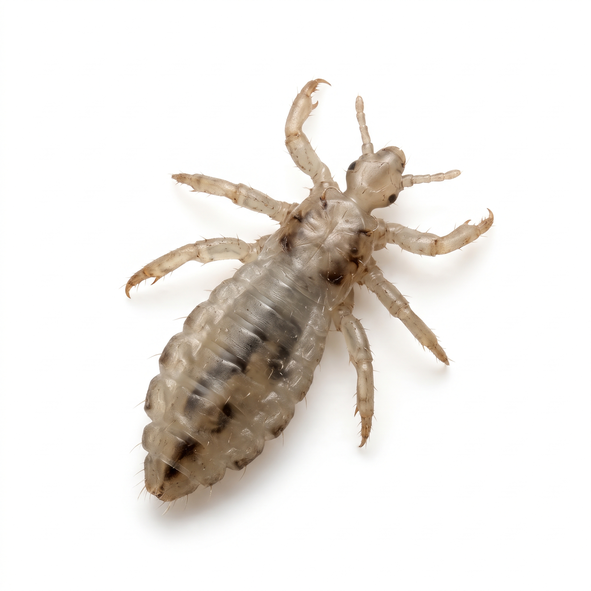
\includegraphics[width=0.85\linewidth]{vokab_300dpi/laus.png} \\
            \vspace{0.3cm}
    }}
    \vspace{0.4em}
    \textbf{\Large D'Laus (Pl. d'Lais)}\\
    \small\textit{(Le pou / The louse)}
\end{minipage}
\hfill
\begin{minipage}[t]{0.48\textwidth}
    \centering
    \textbf{\Large E Mier}
    \vspace{0.4em}
    \framebox{\parbox{0.88\linewidth}{\centering
            \vspace{0.3cm}
            
\includegraphics[width=0.85\linewidth]{vokab_300dpi/mier.png} \\
            \vspace{0.3cm}
    }}
    \vspace{0.4em}
    \textbf{\Large D'Mier (Pl. d'Mierer)}\\
    \small\textit{(La mer / The sea)}
\end{minipage}
\end{noindent}
